\newpage
\section{Kalman Filter}

In this section we implement a discrete Kalman filter to estimate the heading $\psi$, the bias $b$ and the high-frequency wave-induced motion on the heading $\psi_{\omega}$. Instead of the compass measurement, we will use the estimated $\psi$ for feedback in the control law, also known as wave filtering.

%%%%%%%%%%%%%%%%%%%%%%%%%%%%%%%%%%%%%%%%%%%
% 5.1 Discretization
%%%%%%%%%%%%%%%%%%%%%%%%%%%%%%%%%%%%%%%%%%%
\subsection{Discretization}
A discrete model of the system is required to implement the discrete Kalman filter. This is done by using the continous state-space model from section 4.1 in MatLab where exact discretization is used along with a sampling frequency of 10Hz. The MatLab script below shows how this is done by discretizing the matrices in two steps with the function $[Ad, Bd] = c2d(A,B,T)$, once with \textbf{B} as input matrix and then once with \textbf{E} considering the white noise \textbf{w} as input.

\textbf{Discretization of model:}
\begin{lstlisting}
f_s=10;         % Sampling frequency [Hz]
T_s = 1/f_s;    % Sampling time [s]

% Discretize model 
[Ad,Bd] = c2d(A,B,T_s);
% Discretize model 
[~,Ed] = c2d(A,E,T_s);
Cd=C;
\end{lstlisting}


Using zero-order hold on the input and sample time T we descitize the matrices as follows:

\begin{equation}\label{discmat}
    \begin{array}{l}
{A_d} = {e^{AT}}\\
{B_d} = \left( {\int\limits_0^T {{e^{A\tau }}d\tau } } \right)B\\
{C_d} = C
\end{array}
\end{equation}

The resulting matrices are shown below:

\begin{equation*}
    {A_d} = \left[ {\begin{array}{*{20}{c}}
{0.9970}&{0.0992}&0&0&0\\
{ - 0.0607}&{0.9836}&0&0&0\\
0&0&1&{0.0999}&0\\
0&0&0&{0.9988}&{ - 0.0002}\\
0&0&0&0&1
\end{array}} \right]
\end{equation*}


\begin{equation*}
    \begin{array}{cc}
       {E_d} = \left[ {\begin{array}{*{20}{c}}
{0.0015}&0\\
{0.0295}&0\\
0&0\\
0&0\\
0&{0.1}
\end{array}} \right]  ,&  
        {B_d} = 1 \cdot {10^{ - 3}} \cdot \left[ {\begin{array}{*{20}{c}}
0\\
0\\
{0.0101}\\
{0.2012}\\
0
\end{array}} \right]
    \end{array}
\end{equation*}

\begin{equation*}
    {C_d} = \left[ {\begin{array}{*{20}{c}}
0&1&1&0&0
\end{array}} \right]
\end{equation*}


%%%%%%%%%%%%%%%%%%%%%%%%%%%%%%%%%%%%%%%%%%%
% 5.2 Estimation of measurement noise variance
%%%%%%%%%%%%%%%%%%%%%%%%%%%%%%%%%%%%%%%%%%%
\subsection{Estimation of measurement noise variance}

By simulating the ship with zero input(no waves or current), and by applying the measurement noise we were able to obtain an estimate of the belonging variance. In theory, this would mean that the ship would keep a constant heading, $\psi = 0$, providing the measurement noise as resulting signal. Below you can see how this was extracted in MatLab.


\begin{lstlisting}

simTime = 600; % [s]
simout = sim('ship5b','startTime','0','stopTime',sprintf('%d',simTime)); % no noise
psi = simout.get('compass'); 
R = var(psi*pi/180);    
\end{lstlisting}

%%%%%%%%%%%%%%%%%%%%%%%%%%%%%%%%%%%%%%%%%%%
% 5.3 Implementing the Kalman Filter
%%%%%%%%%%%%%%%%%%%%%%%%%%%%%%%%%%%%%%%%%%%
\subsection{Implementing the Kalman Filter}

%The Kalman filter were implemented using an s-function setup as a struct in MatLab, with all the discrete-time model matrices, the covariance matrices and the initial conditions.%

The Kalman filter were implemented using a normal MatLab function within the Matlab function Simulink block, according to Appendix B in the assignment text with persistent variables.

In section 5.2 we obtained the variance which in this case is divided by the sample time $T=0.1s$ and used as the variance of the measurement noise in the filter, $E\{v^2\} = R$. To obtain the desirable units for the filter model, conversions are applied inside MatLab and Simulink.

The Kalman filter is defined as:

\begin{equation}\label{Kin}
    {i_{KF}} = {[\begin{array}{*{20}{c}}
\delta &y
\end{array}]^T}
\end{equation}
\begin{equation}\label{Kout}
    {o_{KF}} = {\left[ {\begin{array}{*{20}{c}}
{{\xi _\omega }}&{{\psi _\omega }}&\psi &r&b
\end{array}} \right]^T}
\end{equation}

(\ref{Kin}) defines the input to the Kalman filter, while (\ref{Kout}) defines the output. $p_{ii}$ are diagonal elements of $P_{k}$, which corresponds to the variance of the estimation error of ${{{\hat \psi }_\omega }}$, ${\hat \psi }$ and ${\hat b}$ respectively.

A zero-order hold is applied to the input of the Kalman filter, with the same sampling time used for the discretization. The Kalman filter block inherits its sampling time from the preceding block, and even though the Kalman filter runs in $10Hz$, the filter model from section 5.1 is still valid. 
The Kalman filter equations are written in a matlab function called, defined as 

\begin{equation}
   {K_k} = P_k^ - {C^T}{(CP_k^ - {C^T} + R)^{ - 1}}
\end{equation}

\begin{equation}
    {{\hat x}_k} = \hat x_k^ -  + {K_k}({y_k} - C\hat x_k^ - )
\end{equation}

\begin{equation}
    {P_k} = (I - {K_k}C)P_k^ - {(I - {K_k}C)^T} + {K_k}RK_k^T
\end{equation}

\begin{equation}
    {{\hat x}_{k + 1}} = A{{\hat x}_k} + B\delta 
\end{equation}

\begin{equation}
    P_{k + 1}^ -  = A{P_k}{A^T} + EQ{E^T}
\end{equation}


\newpage
%%%%%%%%%%%%%%%%%%%%%%%%%%%%%%%%%%%%%%%%%%%
% 5.4 Feed forward from estimated bias
%%%%%%%%%%%%%%%%%%%%%%%%%%%%%%%%%%%%%%%%%%%
\subsection{Feed forward from estimated bias}
A feed forward is made from the estimated bias to cancel the bias due to current. This implies that the rudder input is now the output of the PD-controller plus the estimated bias $\hat b$. Figure \ref{plot:5d} shows the response of the ship when ${\psi _r} = 30$ and current disturbance is applied. Comparing this response with Figure \ref{plot:3c}, we could clearly see that the feed forward cancels the bias, and the ship is able to slowly reach its desired heading reference. The rudder input is still oscillating due to measurement noise in the feedback loop. 

Figure 11 shows that the bias estimate converges in a satisfying way, and how the rudder input oscillates.

\begin{figure}[!htb]
    \caption{Estimated bias and rudder input $\hat b$}
    \centering
     \centerline{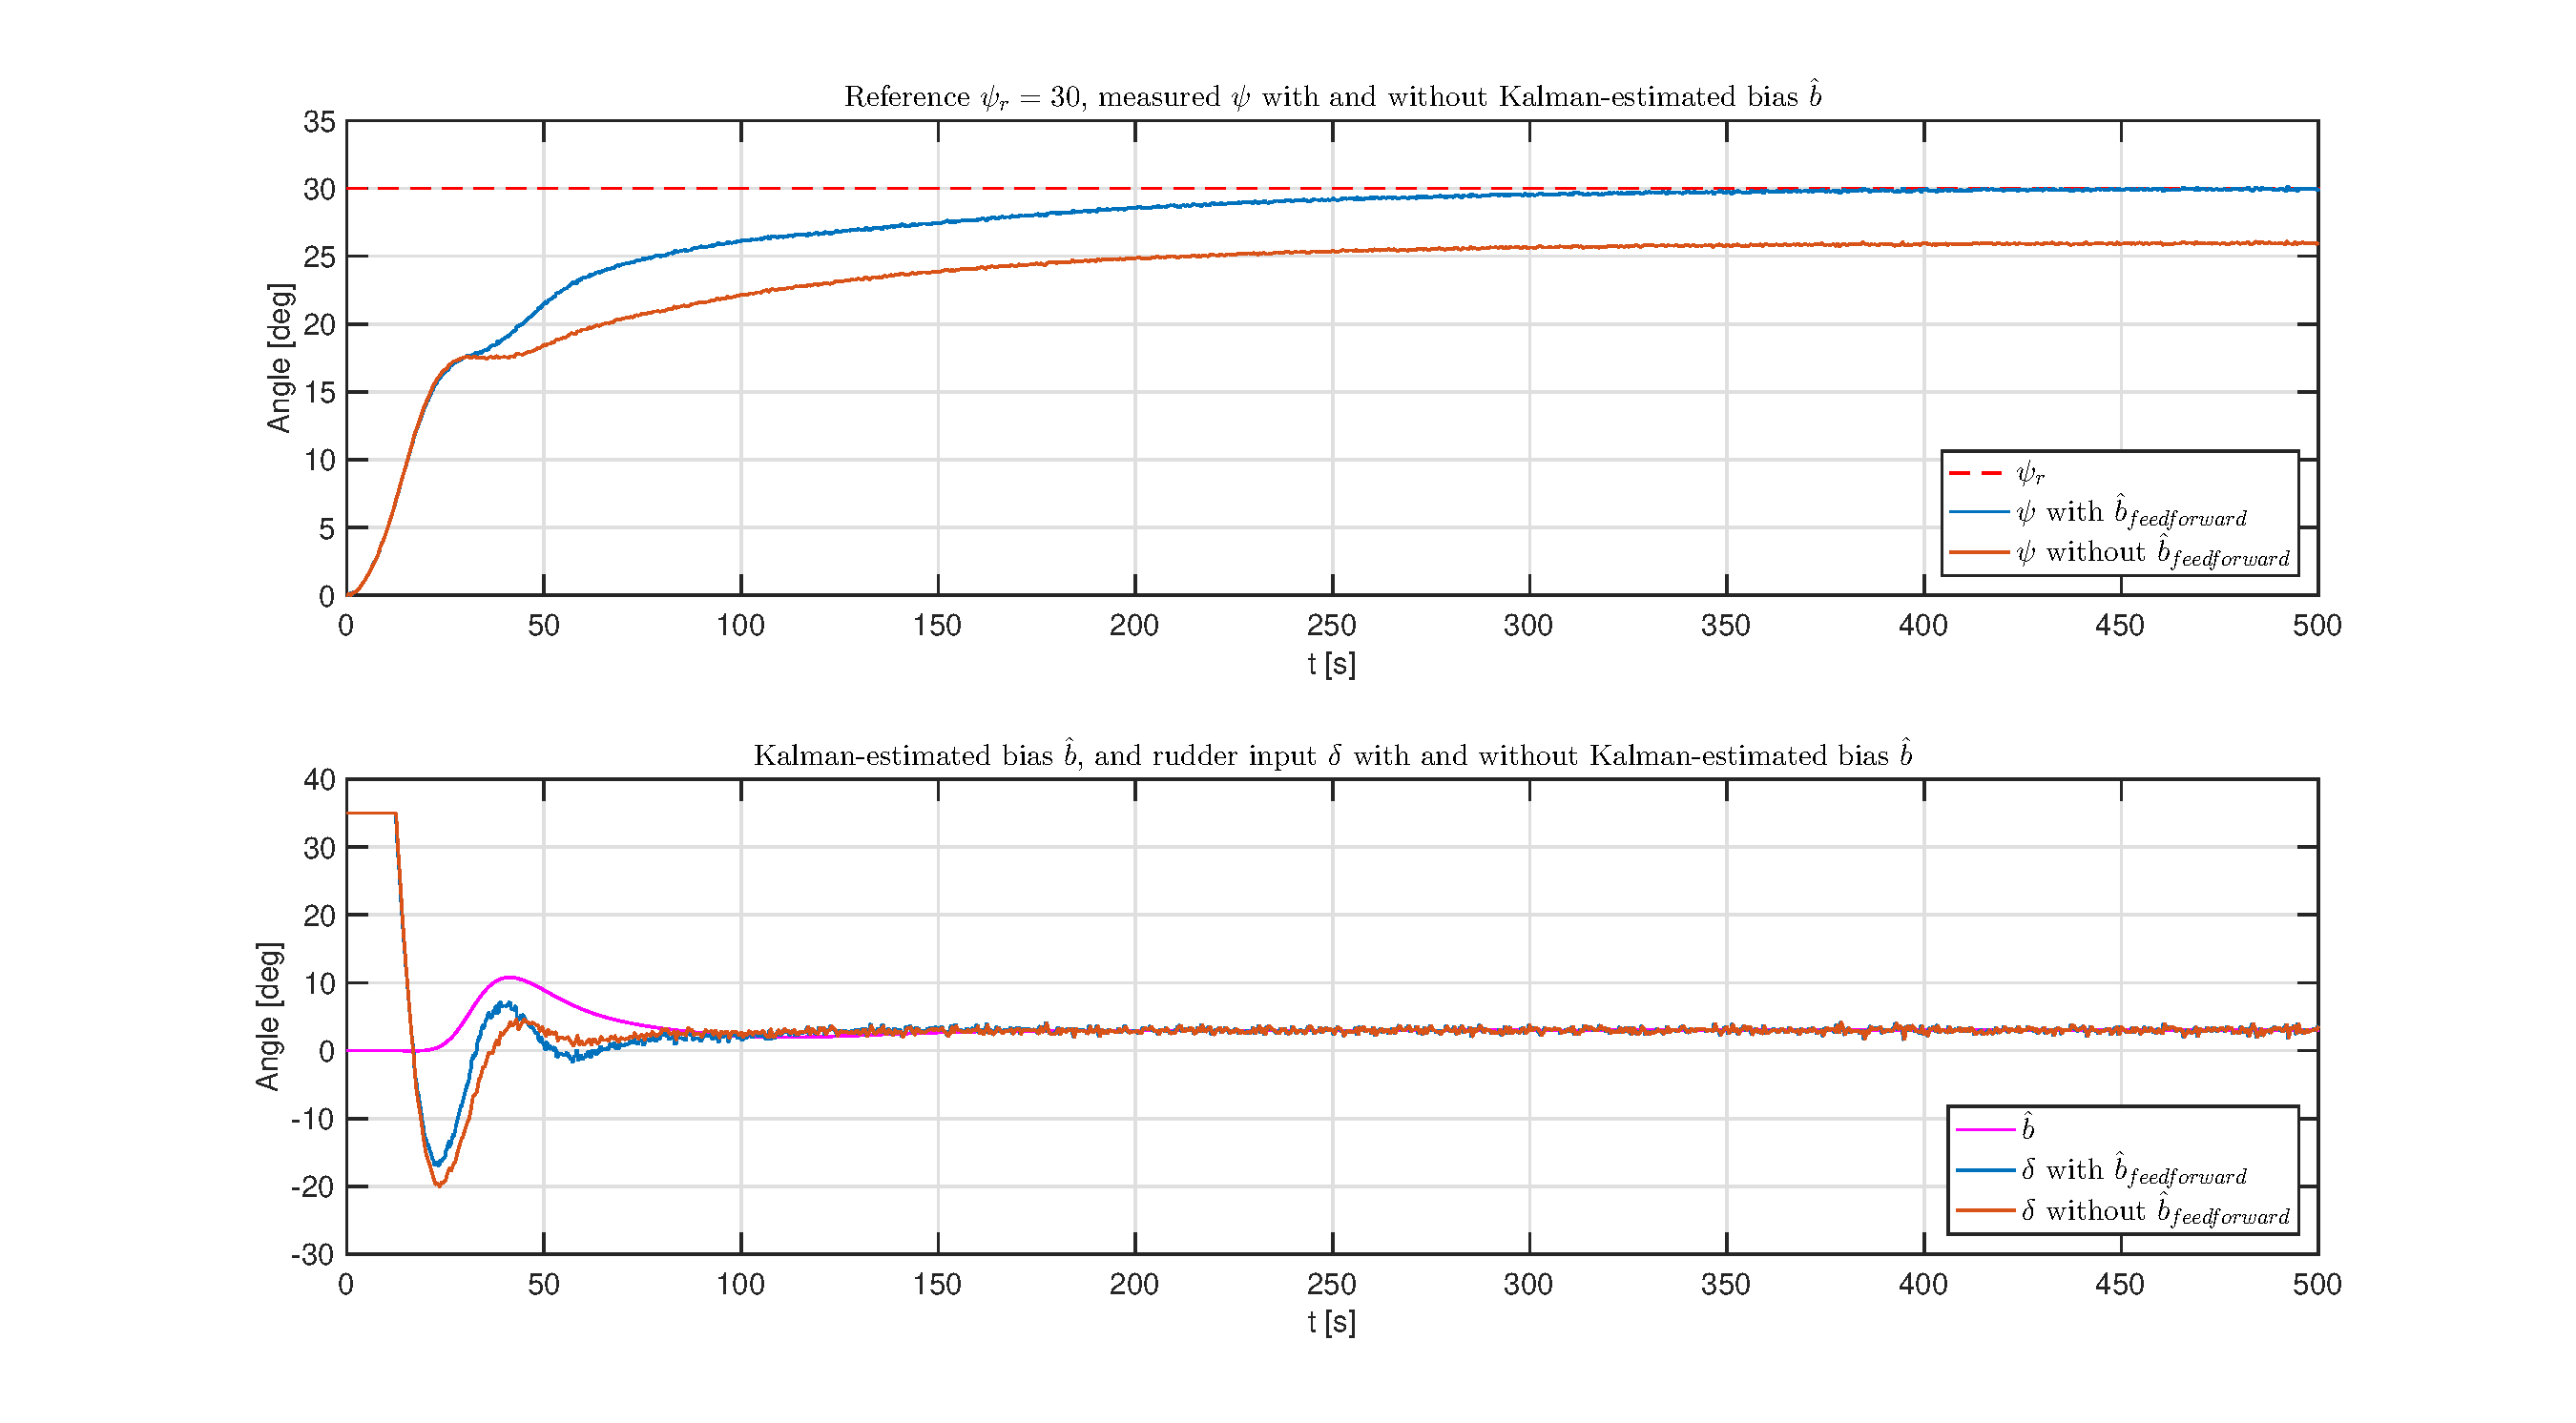
\includegraphics[scale=0.45]{plots/5d}}
    \label{plot:5d}
\end{figure}

\newpage
\begin{figure}[!htb]
    \caption{North-East plot of ship course with and without Kalman}
    \centering
     \centerline{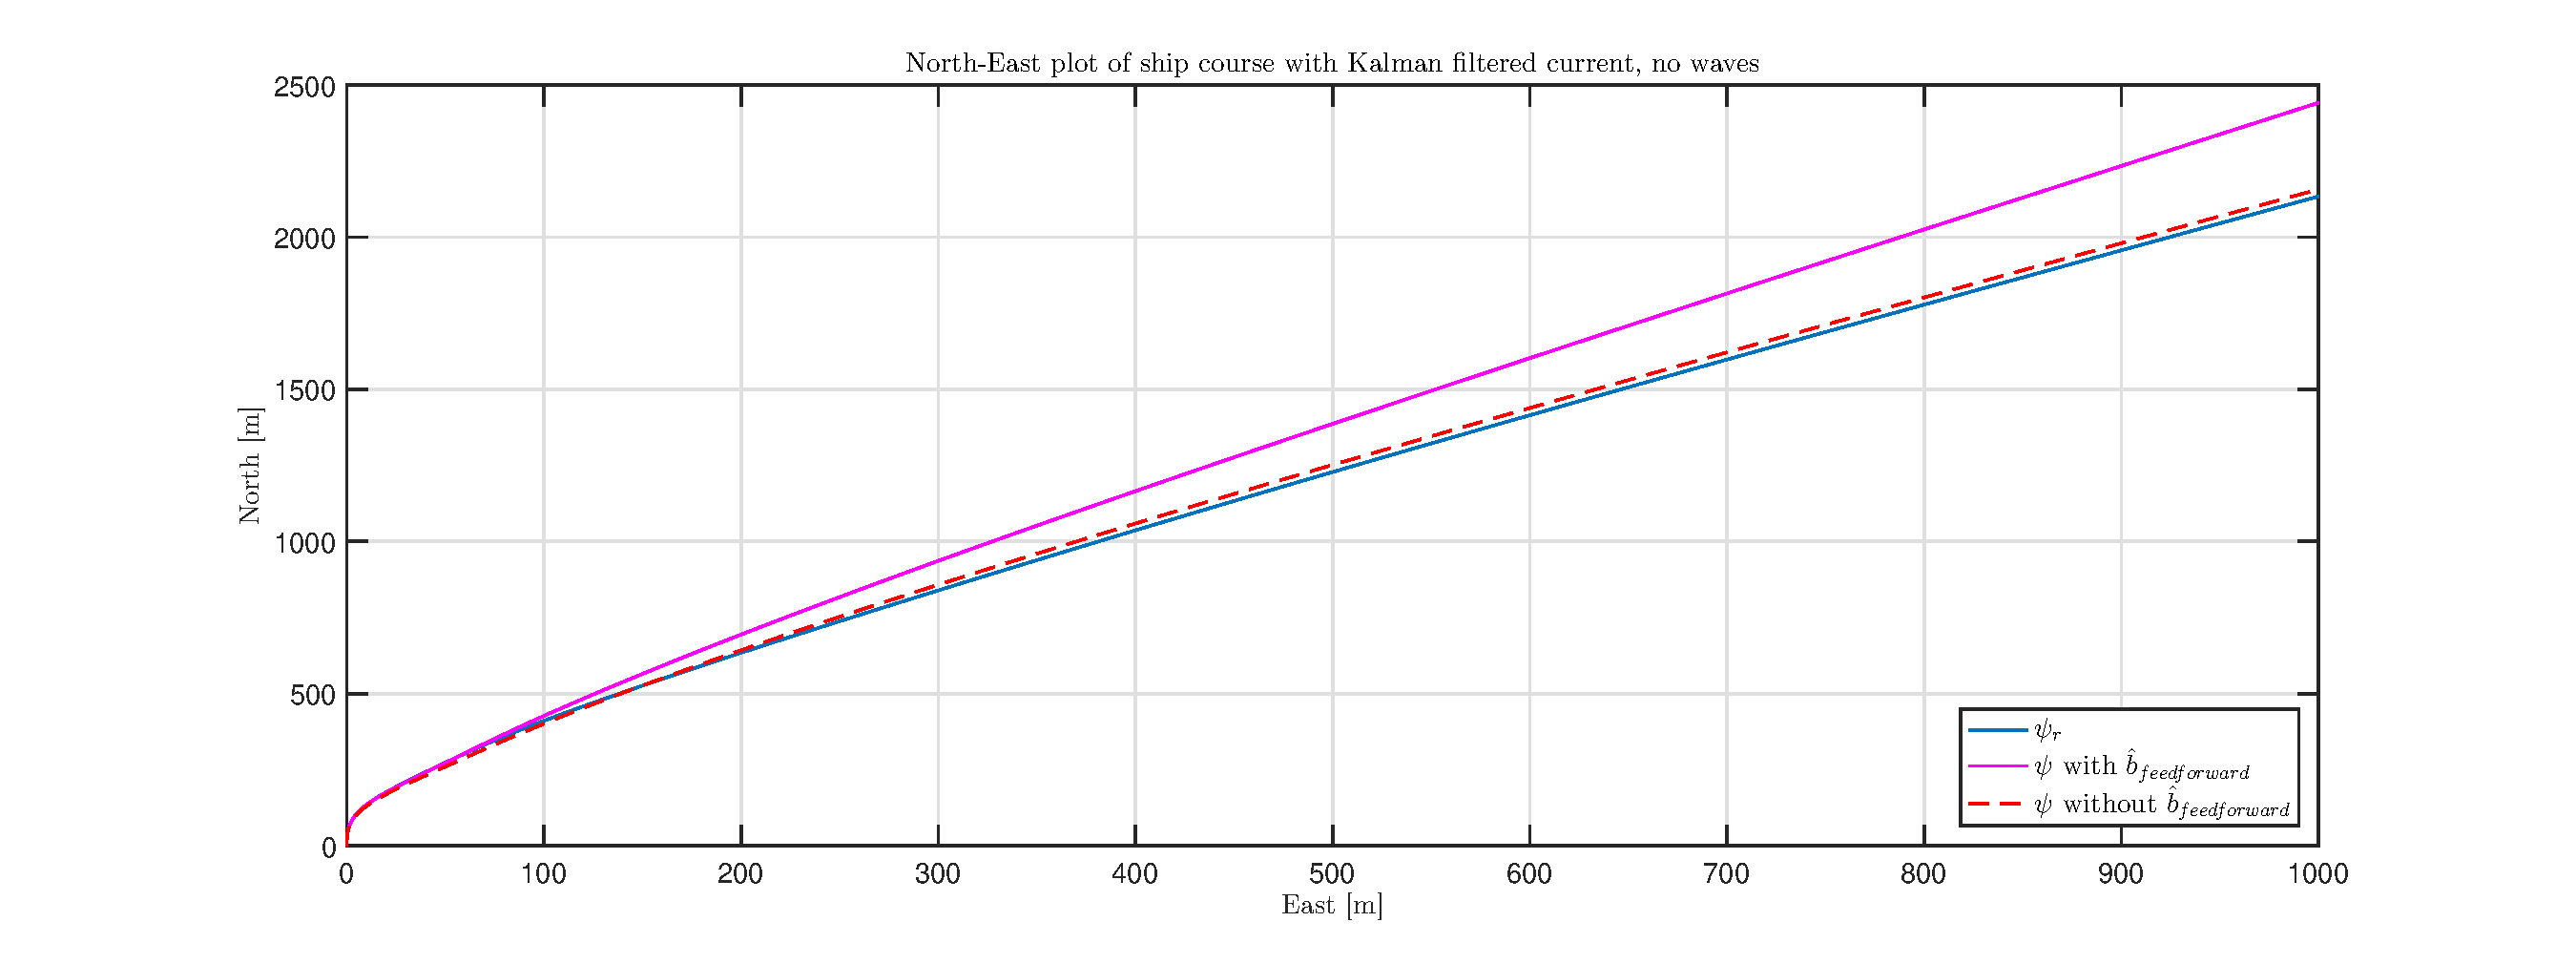
\includegraphics[scale=0.45]{plots/5eORd}}
    \label{plot:5d}
\end{figure}


%%%%%%%%%%%%%%%%%%%%%%%%%%%%%%%%%%%%%%%%%%%
% 5.5 Wave filtering
%%%%%%%%%%%%%%%%%%%%%%%%%%%%%%%%%%%%%%%%%%%
\subsection{Wave filtering}

In this section, the estimated heading $\hat \psi $ will be used instead of the measured heading for the feedback in the autopilot, in addition to the feed forward from the estimated bias. This system is also simulated with ${\psi _r} = 30$, but now with both current and wave disturbances applied.
From Figure 13 we can see the estimated compass $\hat{\psi}$ and the measured compass $\psi$, with the estimated having much less oscillations. In Figure 14 we can see the rudder input and estimated bias, with and without Kalman. Figure 15 shows the heading of the ship with and without Kalman, while Figure 16 shows that the wave bias estimator follows the measured bias, meaning we have a good estimator. 

\begin{figure}[!htb]
    \caption{Measured compass and estimated compass}
    \centering
    \centerline{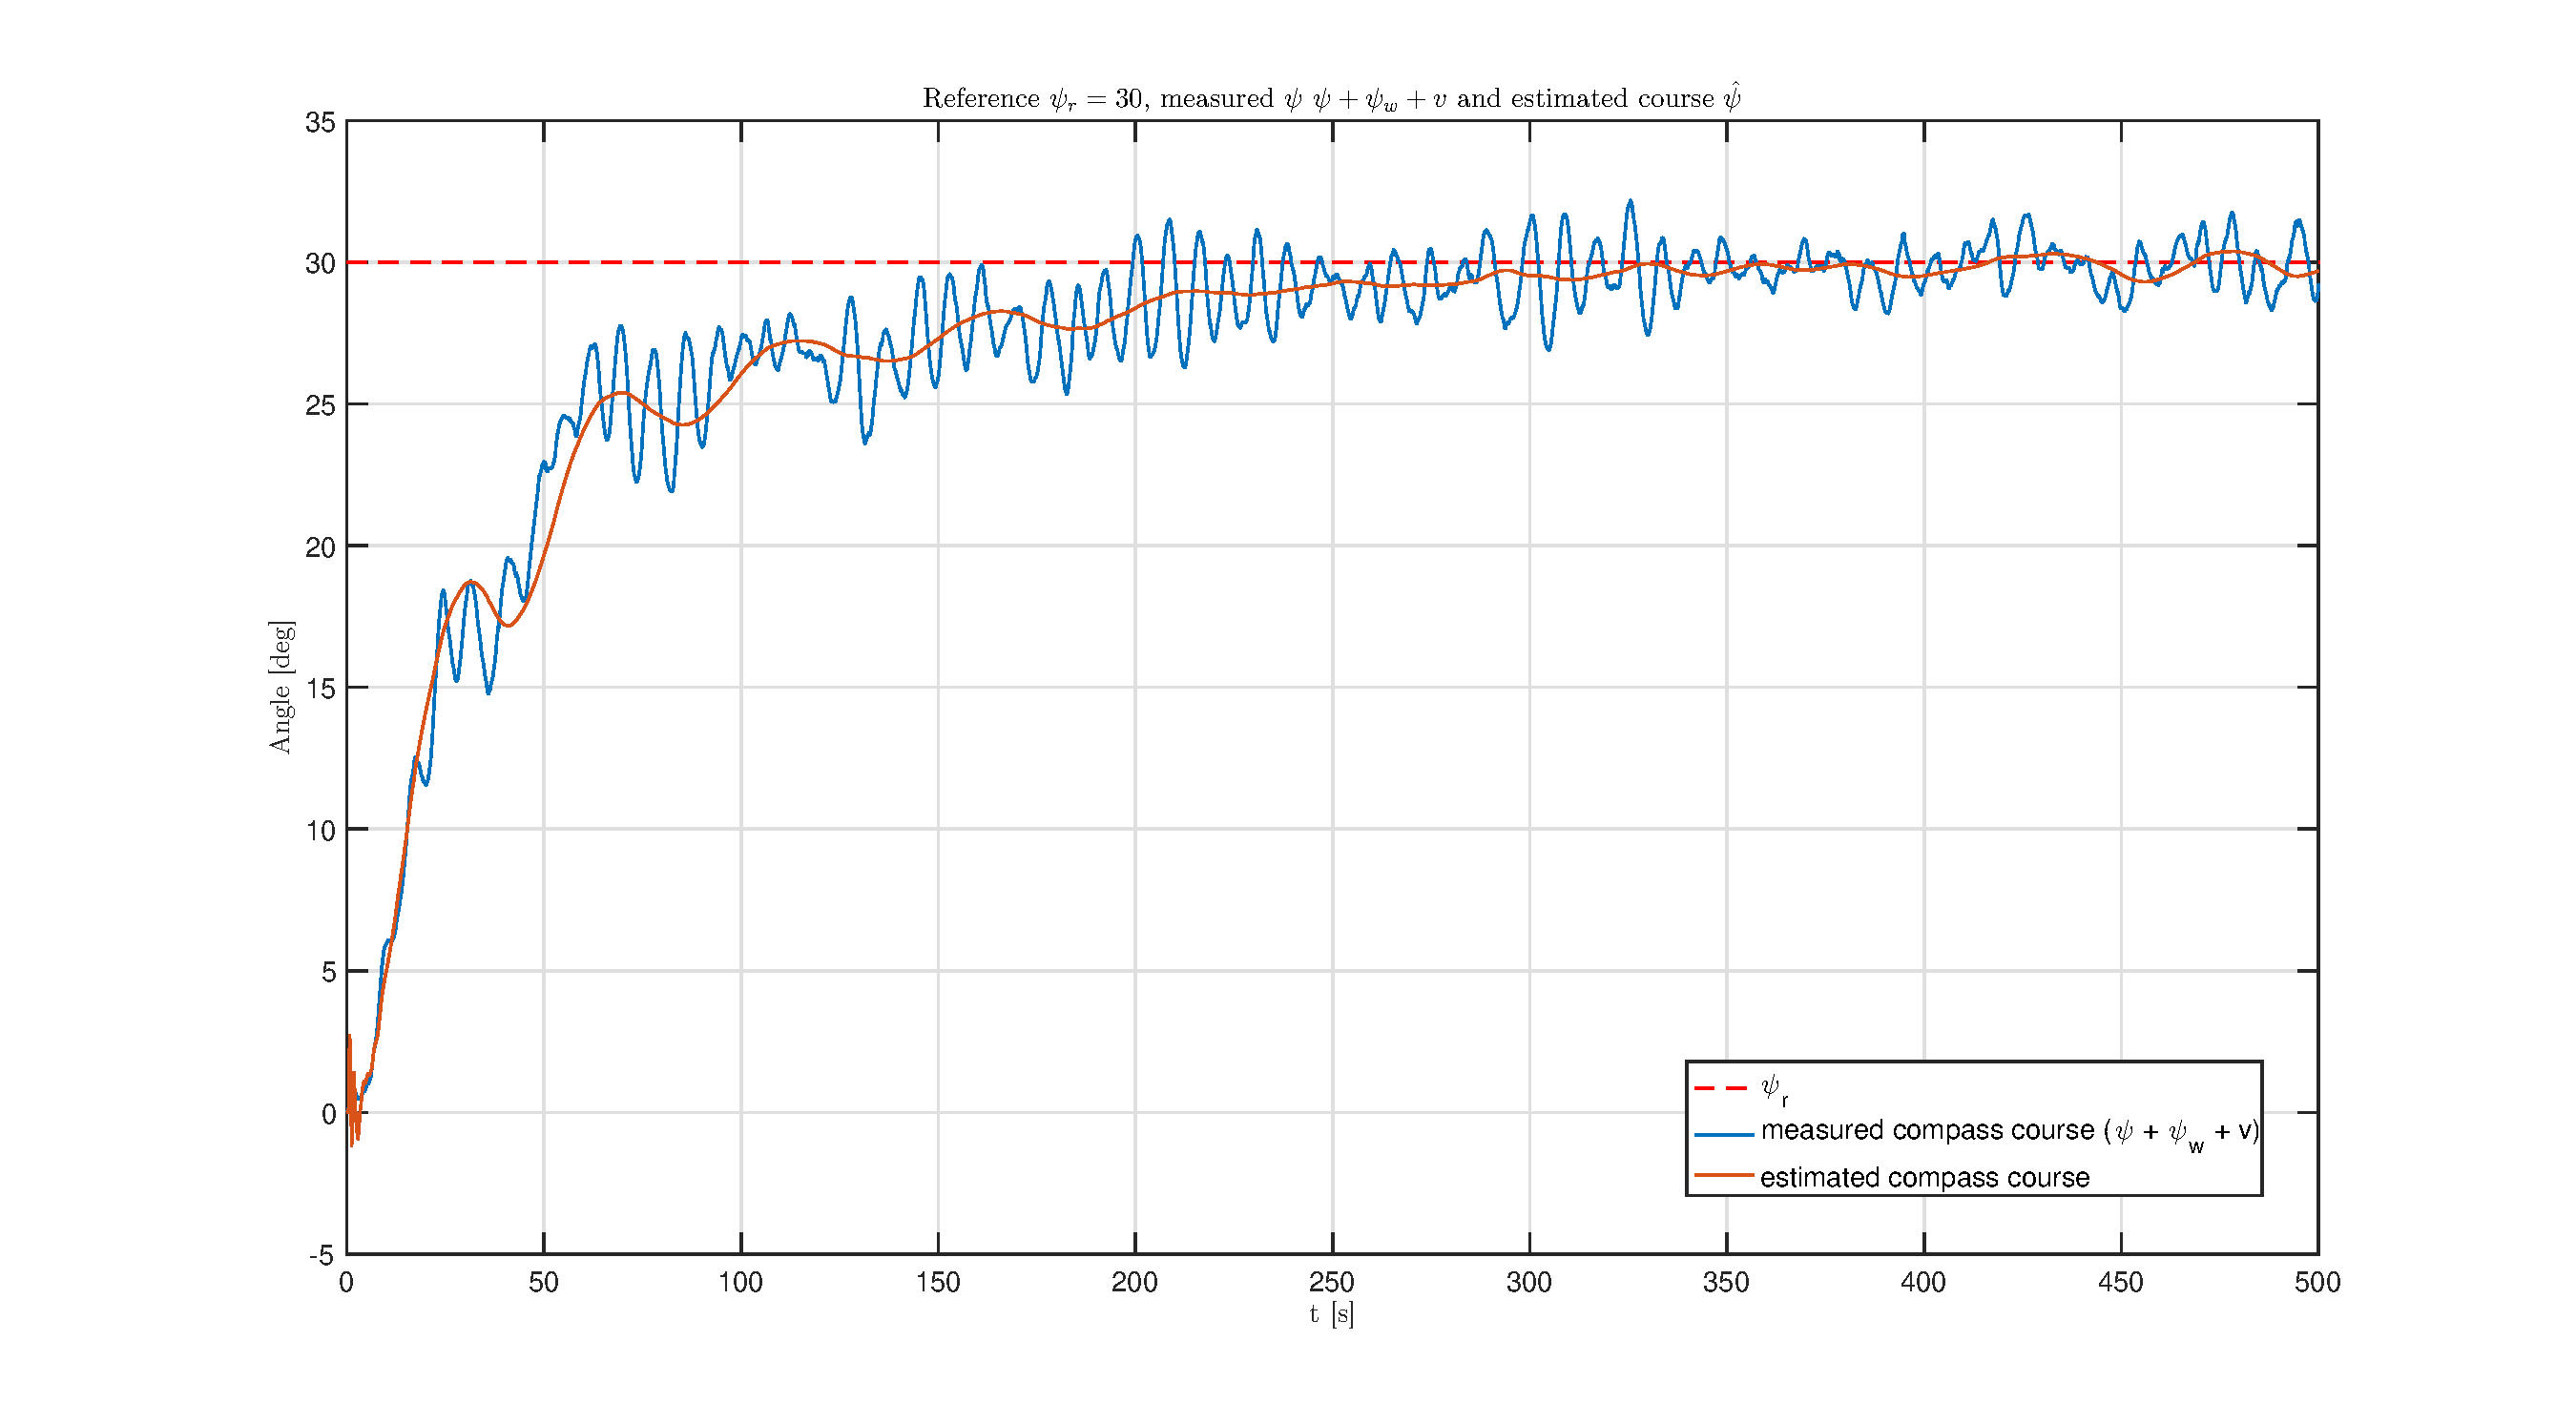
\includegraphics[scale=0.25]{plots/5e5}}
    \label{plot:5e1}
\end{figure}


\begin{figure}[!htb]
    \caption{Rudder input and estimated bias}
    \centering
    \centerline{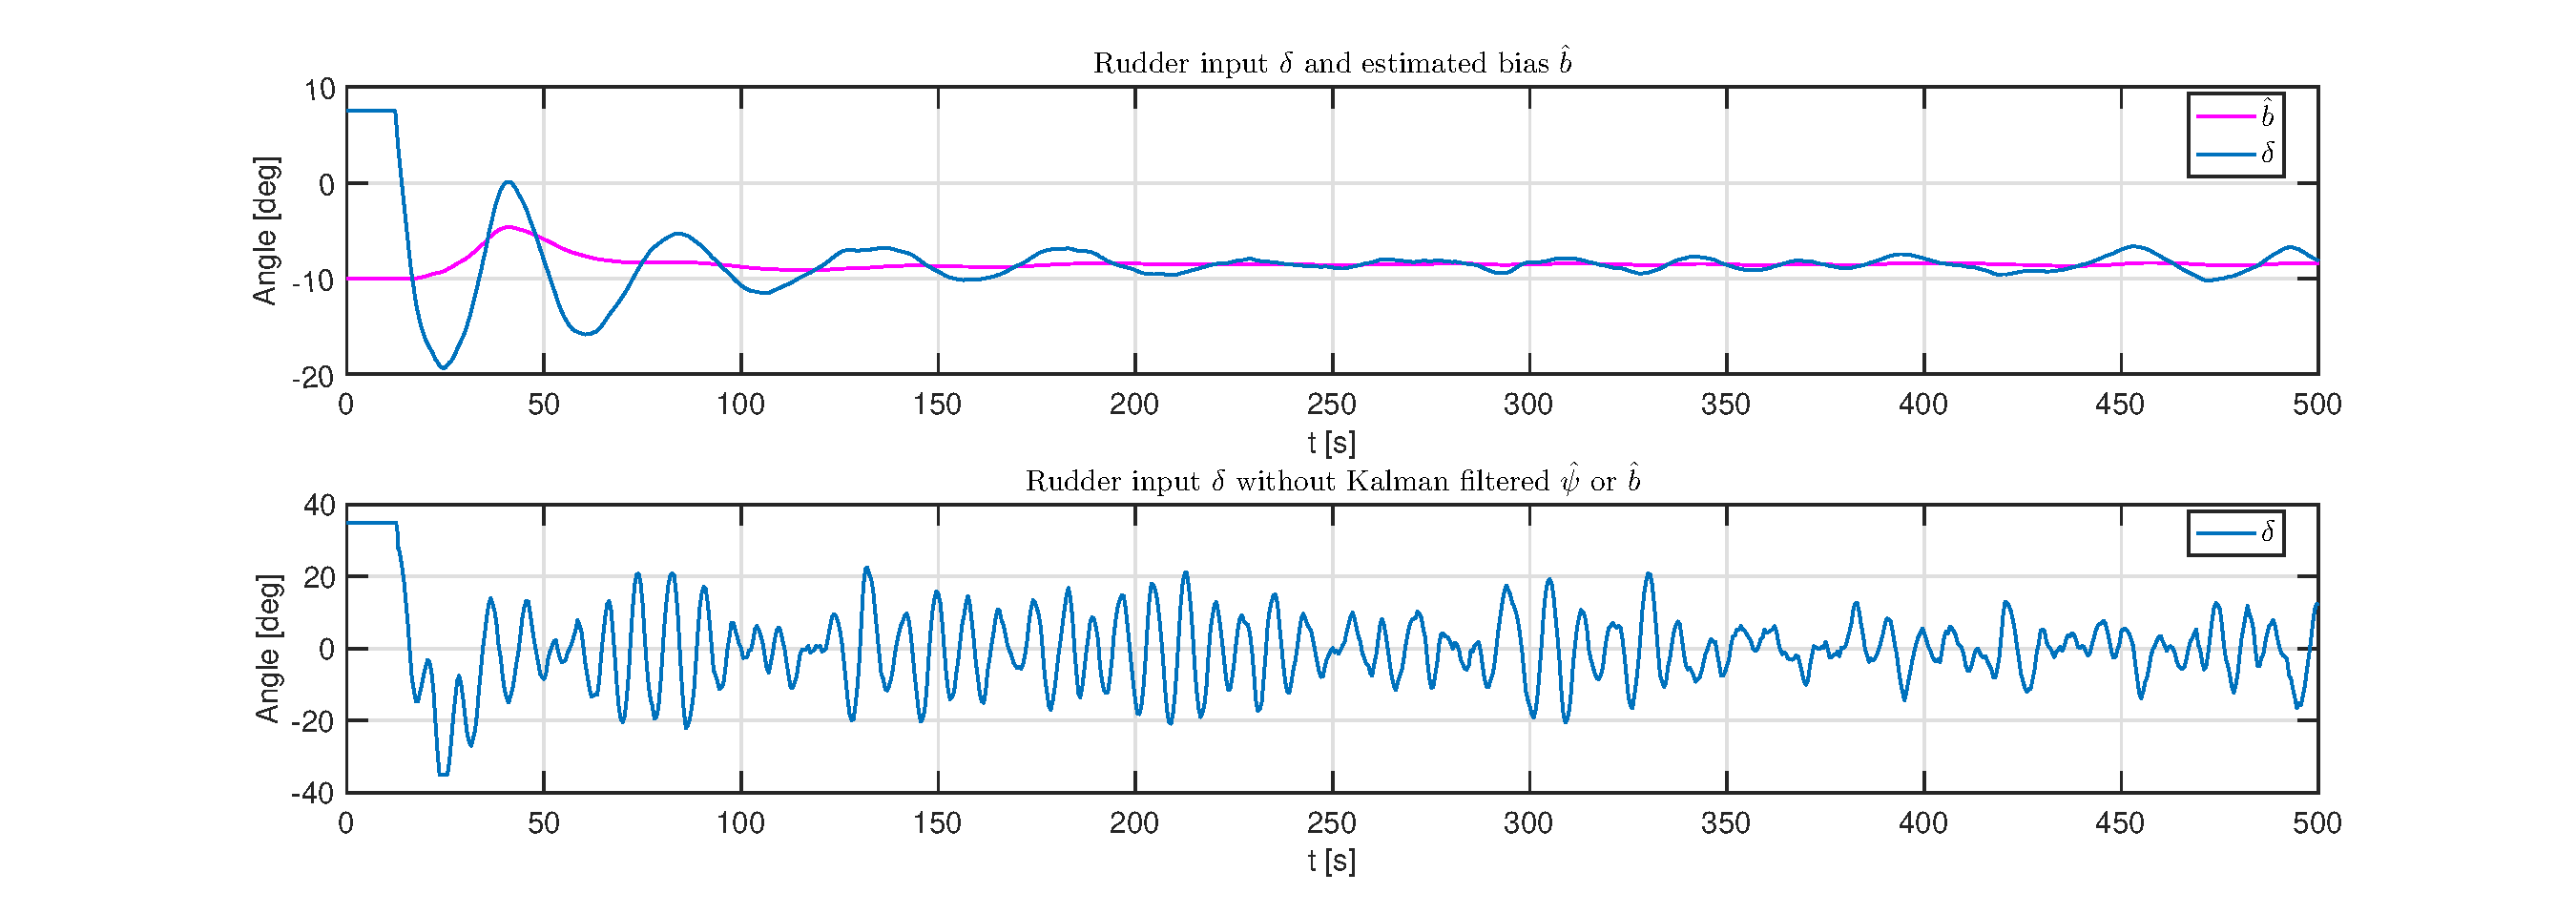
\includegraphics[scale=0.40]{plots/5e1}}
    \label{plot:5e1}
\end{figure}

\begin{figure}[!htb]
    \caption{North-East plot with Kalman filtered current and waves}
    \centering
    \centerline{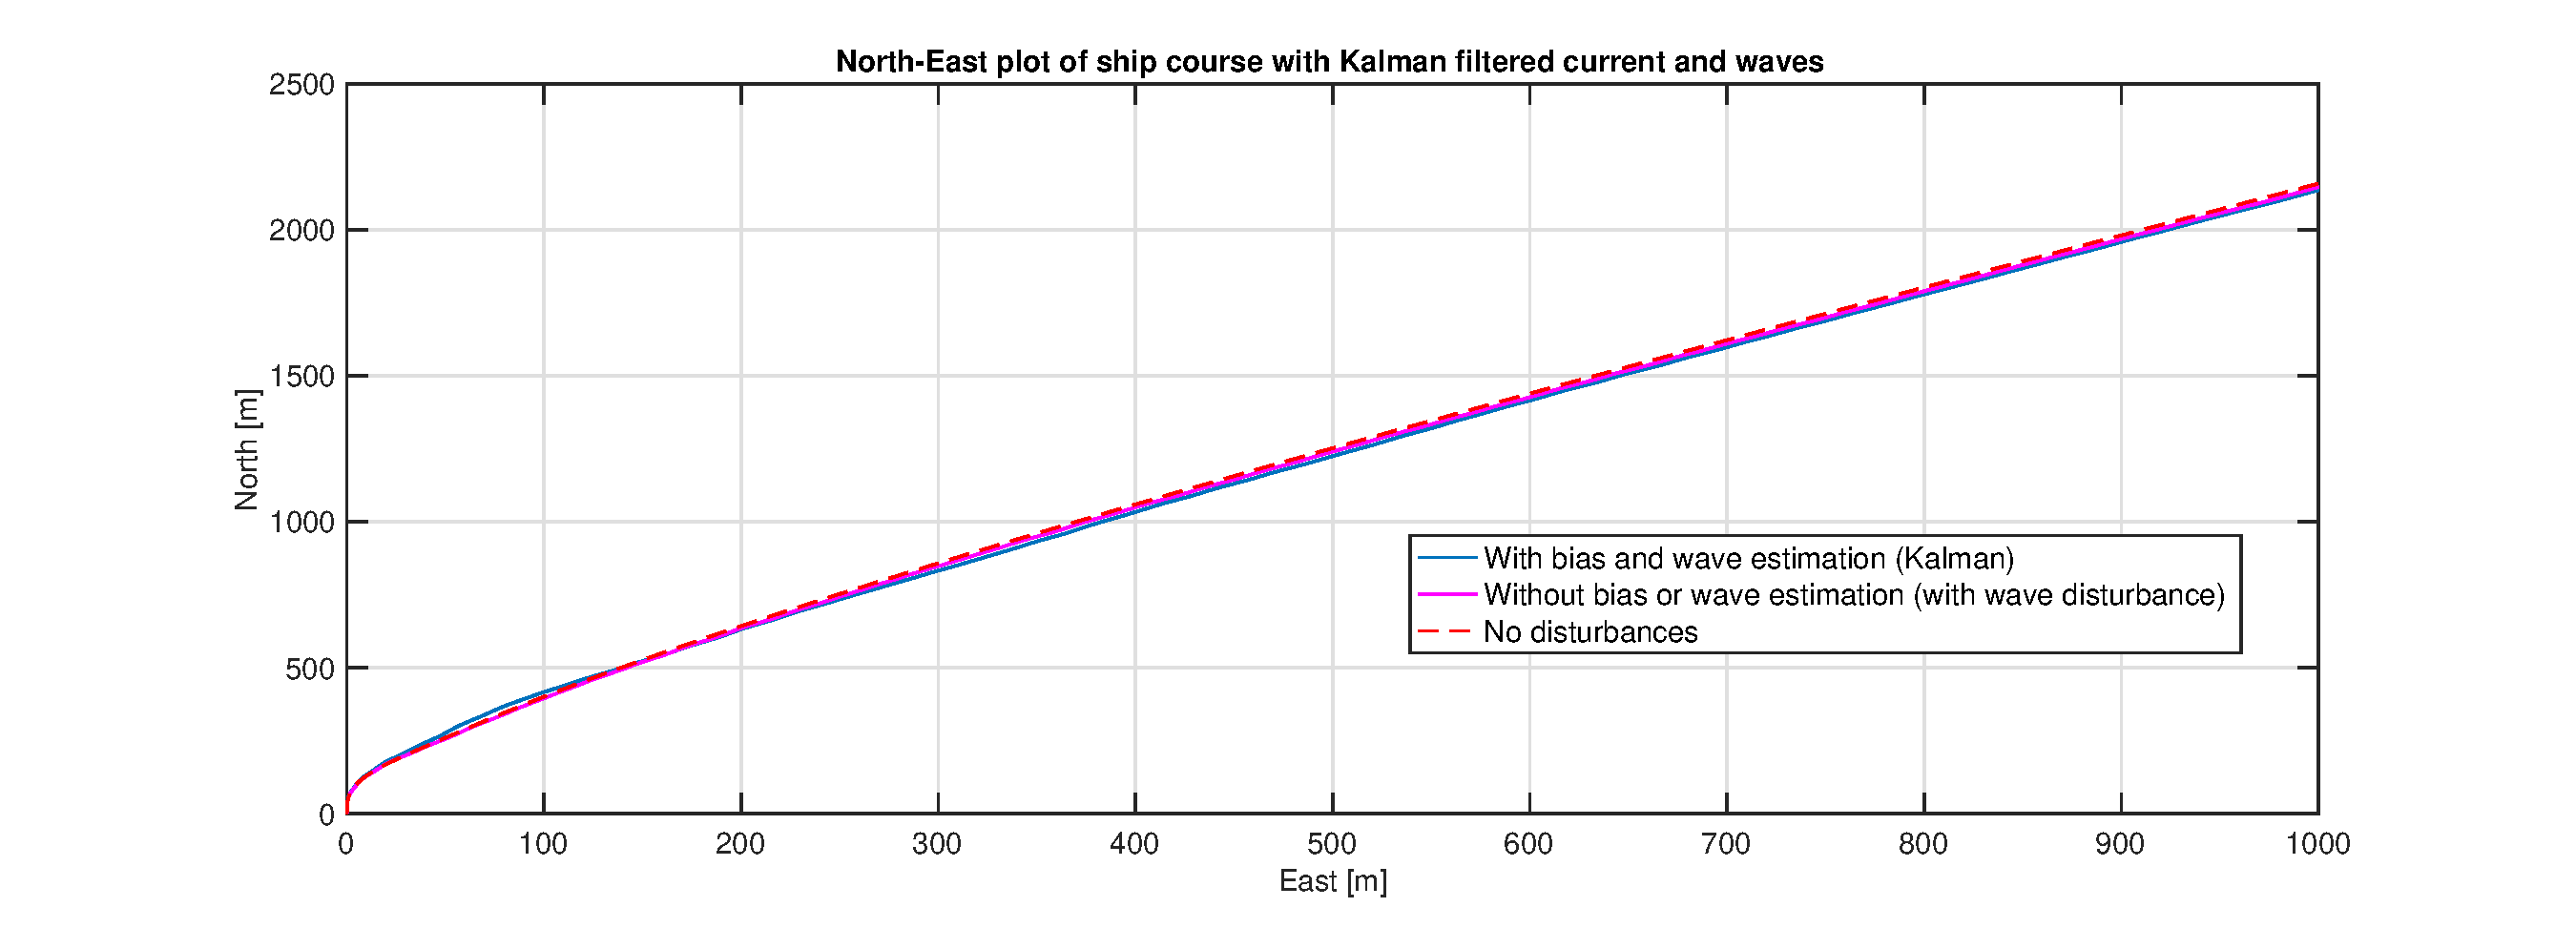
\includegraphics[scale=0.35]{plots/5e2}}
    \label{plot:5e2}
\end{figure}

\begin{figure}[!htb]
    \caption{Wave influence}
    \centering
    \centerline{\includegraphics[scale=0.30]{plots/5e3}}
    \label{plot:5e3}
\end{figure}

\newpage\null\thispagestyle{empty}\newpage